%!TEX root = ..\main.tex
%!TEX encoding = UTF-8 Unicode

%——————————————————————————————————————————————————————————-
%	CHAPTER 12
%   Translator:SI
%   Proofread : lh1962
%——————————————————————————————————————————————————————————-

\chapterimage{chapter_head_1.pdf} % Chapter heading image

\chapter[引力]{Gravity \quad 引力}
\label{chap12}
{\it 非常不幸,目前最靠谱的引力理论与本书其他部分(对称性)的三观不合。这是现代物理学的最大问题之一,本章尝试使读者对这一疑难有所认识。}

现代的引力理论是{\bf Einstein}的{\bf 广义相对论(general relativity)}。广相的基本思想是引力为时空弯曲的结果。质量/能量改变时空的曲率,变化了的曲率进而影响质量/能量的运动。能量与曲率的这一互动由著名的Einstein场方程描述:
\begin{equation}
\label{equ12.1}
    G_{\mu \nu} = 8 \pi G T_{\mu \nu}.
\end{equation}
等号左侧是描述曲率的Einstein张量$G_{\mu \nu}$,右侧是能量-动量张量%
\mpar{能量-动量张量是与平移对称性直接相关的量,见\ref{equ4.36}式。}%
$T_{\mu \nu}$,$G$是引力常数。

在现代观点——引力 = 时空曲率的指导思想下,Einstein场方程的形式比较容易导出%
\mpar{100年前,Einstein经过大概6年导出了场方程的正确形式。100年后,在现代的较高观点之下,场方程的导出更加直接明快。}%
。怎么导出?首先,能量-动量守恒是最重要的物理定律之一,这可以从时空的均匀性直接推导(见第四章),在均匀时空中物理规律在时空的平移变换下不变。因此,将时空的均匀性作为基本假设的话,能量与动量自然就是守恒的,这一守恒定律的数学形式为(\ref{equ4.36}式):
\begin{equation}
\label{equ12.2}
    \partial^\mu T_{\mu \nu} = 0.
\end{equation}
下面介绍描述关于曲率的数学工具,它是广义相对论繁琐计算的根源。我们已经见过关于曲率的重要的量——度规,它用于计算两点间距离%
\mpar{目前为止用到的度规包括 Minkowski 度规$\eta^{\mu \nu} = \begin{pmatrix} 1 & 0 & 0 & 0 \\ 0 & -1 & 0 & 0 \\ 0 & 0 & -1 & 0 \\ 0 & 0 & 0 & -1 \end{pmatrix}$和 Euclidean 度规$\delta^{ij} = \begin{pmatrix} 1 & 0 & 0 \\ 0 & 1 & 0 \\ 0 & 0 & 1 \end{pmatrix}.$}%
。由图\ref{fig12.1}可见,弯曲空间中的两点间距与平直时空的两点不同,因而度规在曲率的数学描述中起到十分重要的作用。

\marginpar{
	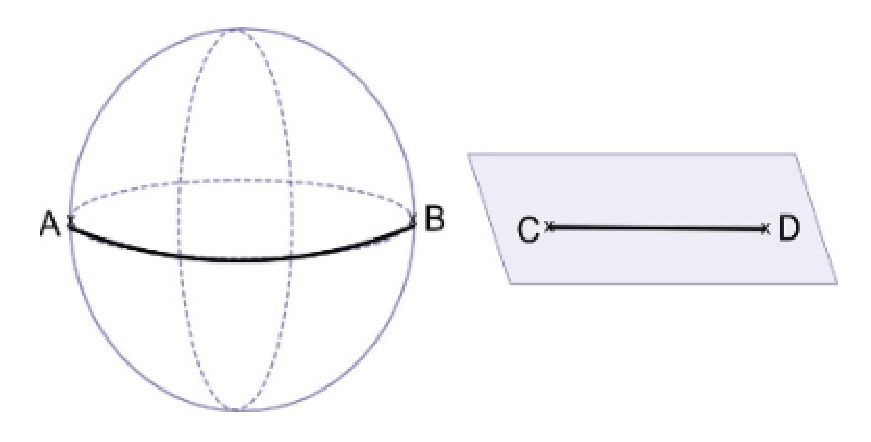
\includegraphics[scale=0.35]{fig12_1.eps}
	\figcaption{弯曲空间与平直空间中的两点间距}
    \label{fig12.1}
}

现在就能“导出” Einstein 场方程了,因为能放在能动张量对面的量只有一个:Einstein张量$G_{\mu \nu}$。这是因为 Einstein 张量是度规$g_{\mu \nu}$及其一阶、二阶导数的函数中唯一\footnote{译注:至多差一常数与度规张量的乘积,即著名的宇宙学常数$Lambda$} 的无散度%
\mpar{即$\partial^\mu G_{\mu \nu} = 0$.}%
函数。不管其多复杂,放到等号一边描述曲率的量只能是它,因为
\begin{equation}
\label{equ12.3}
    T_{\mu \nu} = C G_{\mu \nu}, \quad \text{由} \partial^\mu T_{\mu \nu} = 0 \to \partial^\mu G_{\mu \nu} = 0.
\end{equation}
Einstein 张量是二阶张量%
\mpar{二阶张量是指它有两个指标$\mu \nu$,这与散度为零一样也是限制之一,因为$T_{\mu \nu}$是二阶张量。}%
,正好符合要求。

Einstein张量通过Ricci张量$R_{\mu \nu}$、Ricci标量$R$(即Ricci张量的迹:$R \equiv R^\nu_\nu$)和度规张量$g_{\mu \nu}$定义:
\begin{equation}
\label{equ12.4}
    G_{\mu \nu} = R_{\mu \nu} - \frac{1}{2} R g_{\mu \nu}.
\end{equation}
其中Ricci张量由Christoffel符号$\Gamma^\mu_{\nu \rho}$定义:
\begin{equation}
\label{equ12.5}
    R_{\alpha \beta} = \partial_\rho \Gamma^\rho_{\beta \alpha} - \partial_\beta \Gamma^\rho_{\rho \alpha} + \Gamma^\rho_{\rho \lambda} \Gamma^\lambda_{\beta \alpha} - \Gamma^\rho_{\beta \lambda} \Gamma^\lambda_{\rho \alpha}
\end{equation}
其中 Christoffel 符号通过度规张量定义:
\begin{equation}
\label{equ12.6}
    \Gamma^d_{ab} = \frac{1}{2} g^{cd} \left( \frac{\partial g_{ca}}{\partial x^b} + \frac{\partial g_{cb}}{\partial x^a} - \frac{\partial g_{ab}}{\partial x^c} \right) = \frac{1}{2} g^{cd} (\partial_b g_{ca} + \partial_a g_{cb} - \partial_c g_{ab}).
\end{equation}
上面的式子复杂得吓人,这稍微揭示了广义相对论计算的繁复程度。

现在考虑物体在弯曲时空中的行为。设自由物体经过弯曲时空中的$A, B$两点,物体在$A, B$之间的轨迹是怎样的?容易猜想物体沿弯曲时空中两点间的最短路径(称为短程线)运动,确实如此(证明略)。这样,给定质能分布$T_{\mu \nu}$之后就可根据Einstein场方程计算度规与Christoffel符号,从而得到自由质点的轨迹——{\bf 短程线方程(geodesic equation)}:
\begin{equation}
\label{equ12.7}
    \frac{d^2 x^\lambda}{dt^2} + \Gamma^\lambda_{\mu \nu} \frac{d x^\mu}{dt} \frac{d x^\nu}{dt} = 0.
\end{equation}
测地线是流形上的两点间局域最短%
\mpar{这一说法是过于简单的,正确的概念需要微分几何的相关知识,超出本书范围。}%
的连线。

有趣的是,Einstein将Christoffel符号视作引力场%
\mpar{一般将度规视为引力场。}%
:
\begin{quote}
若$\Gamma^\mu_{\nu \rho}$消失,则(自由)质点沿直线匀速运动,因此$\Gamma^\mu_{\nu \rho}$描述了关于匀速直线的偏离,它们是引力场的分量。
\end{quote}
\begin{flushright}
-- {\bf Albert Einstein}\mpar{Albert Einstein. The foundation of the general theory of relativity. 1916}
\end{flushright}
从\ref{equ12.7}式就能理解Einstein所说的,令$\Gamma^\mu_{\nu \rho} = 0$,测地线方程退化为:
\begin{equation}
\label{equ12.8}
    \frac{d^2 x^\lambda}{dt^2} = 0.
\end{equation}
方程的解是一条直线。

弯曲时空的另一有趣事实是微分符号的变化。平直时空中的导数利用下式定义:
\begin{equation}
\label{equ12.9}
    f'(a) = \lim_{h \to 0} \frac{f(a + h) - f(a)}{h}.
\end{equation}
上式用到了函数$f$在两个不同点的值。弯曲时空的情形不像平直时空那样简单。如图12.2,如果想比较球面上不同位置的两个向量的差值,怎样才能得到它们真正的差而除去弯曲空间造成的影响?微分几何告诉我们可以进行平移,将一个向量平移到另一个向量的位置,从而可以%
\mpar{实际上,微分几何中的坐标系都是局域的。\ref{sec3.11}节讲过,流形的主要特征是局域平直(像Euclidean空间)。因此,流形上对象的坐标只在一个坐标域内有效,同样只能在同一坐标域内比较不同对象的坐标差值。}%
比较它们。

\marginpar{
	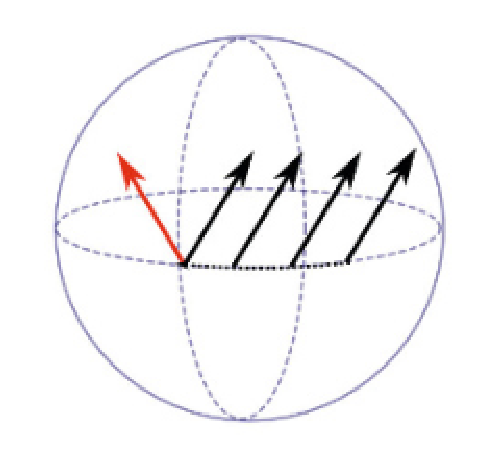
\includegraphics[scale=0.5]{fig12_2.eps}
	\figcaption{为了比较红色箭头与黑色箭头,我们将黑色箭头平移到红色箭头的位置。}
}

弯曲空间中的导数称为{\bf 协变导数 (covariant derivative)}%
\mpar{这里的Christoffel符号$\Gamma^a_{\phantom{a}bc}$通常称为联络系数,因为它们联系了进行比较的两点。}%
:
\begin{equation}
\label{equ12.10}
    D_b v^a \equiv \partial_b v^a + \Gamma^a_{\phantom{a}bc} v^c.
\end{equation}
因此,弯曲时空中的方程需要将普通导数替换为协变导数:
\begin{equation}
\label{equ12.11}
    \partial_b \to D_b = \partial_b + \Gamma^a_{\phantom{a}bc}.
\end{equation}
这很眼熟。见\ref{equ7.18}式,我们在先前的章节中讲过,自旋$0$或自旋$\frac{1}{2}$场拉格朗日量的局域$\mathcal{U}(1)$不变性要求与自旋$1$的场有特定的耦合。这一耦合可以用下式描述:
\begin{equation}
\label{equ12.12}
    \partial_\mu \to D_\mu \equiv \partial_\mu + i \mathrm{e} A_\mu.
\end{equation}
注意这不只是个数学技巧,它导出了正确的电磁学理论。弱相互作用的情形也类似:
\begin{equation}
\label{equ12.13}
    \partial_\mu \to D_\mu \equiv \partial_\mu + i g \underbrace{W_\mu}_{\mathclap{= W_\mu^i \sigma^i}}.
\end{equation}
强相互作用也是:
\begin{equation}
\label{equ12.14}
    \partial_\mu \to D_\mu = \partial_\mu + i g' \underbrace{G_\mu}_{\mathclap{= T^C G^C_\mu}}.
\end{equation}
尽管上面各式的形式相似,但引力无法像其他相互作用那样量子化。其他相互作用都是用量子理论描述的,都给出概率性的实验预言。而广义相对论是经典理论,因为广相中的粒子沿确定的轨迹运动,没有概率性因素。

更糟糕的是目前没有任何实验能检测引力与其他力之间的相互作用。基本粒子间的引力太小,无法测量。因此忽视了引力,只考虑强、弱与电磁相互作用的标准模型就可以与实验符合得相当好。大质量物体的广义相对论效应实验上可以测量,但量子效应却十分微弱,因为大质量物体包含大量基本粒子,所有量子效应被平均掉了。第\ref{chap10}章导出了平均值的运动方程,它正是经典物理的形式,毫无量子效应。

引力的量子化的困难可以列出长长的列表,不过Einstein简明地论述了引力与其他相互作用的差异:
\begin{quote}
$\dots$ 根据广义相对论,引力与其他相互作用(特别是电磁力)相比地位特殊,因为描述引力场的十个方程\footnote{或许指Einstein场方程,代表十个方程。——译者}同时确定了时空的度量性质。
\end{quote}
\begin{flushright}
-- {\bf Albert Einstein}\mpar{Albert Einstein and Francis A. Davis.
{\it The Principle of Relativity}. Dover Publications, reprint edition, 6 1952. ISBN 9780486600819}
\end{flushright}

将普通导数替换为协变导数就能描述弯曲时空中的量子粒子,但这并非引力的动力学理论。Einstein场方程等号右侧(能动张量)容易量子化,选定合适的生成元就行了。困难的是等号左边的Einstein张量,它用Christoffel符号写为:
\begin{equation}
\label{equ12.15}
    G_{\alpha \beta} = (\delta^\gamma_\alpha \delta^\zeta_\beta - \frac{1}{2} g_{\alpha \beta} g^{\gamma \zeta}) (\partial_\varepsilon \Gamma^\varepsilon_{\gamma \zeta} - \partial_\zeta \Gamma^\varepsilon_{\gamma \varepsilon} + \Gamma^\varepsilon_{\varepsilon \sigma} \Gamma^\sigma_{\gamma \zeta} - \Gamma^\varepsilon_{\zeta \sigma} \Gamma^\sigma_{\varepsilon \gamma}).
\end{equation}
由此猜想Einstein场方程或许是$\Gamma^\varepsilon_{\zeta \sigma}$的场方程%
\mpar{就像Maxwell方程组与电磁场的关系那样。}%
,并且$\partial_b \to D_b = \partial_b + \Gamma^a_{\phantom{a} bc}$描述引力场$\Gamma^\varepsilon_{\zeta \sigma}$与其他场的耦合。

无论将度规张量(两个指标)还是Christoffel符号(三个指标)视为引力场,描述它们都需要Poincar\'e群的$(1, 1)$以及更高维的表示,或者说自旋$2, 3, \dots$表示。目前大多数物理学家认为引力场量子化后的引力子(graviton)是自旋为$2$的boson。

目前为止,没有靠谱的量子引力理论%
\mpar{许多尝试过程产生了无穷多个无穷大项,这对概率性预言来说十分要命。}%
能比下一节列出教科书上的标准引力理论给出进一步的信息。

\section*{Further Reading Tips \quad 阅读建议}
引力的标准理论——Einstein的广义相对论的更多信息可以参考以下文献:
\begin{itemize}
    \item {\bf  Ta-Pei Cheng - Relativity, Gravitation and Cosmology}%
    \mpar{Ta-Pei Cheng. {\it Relativity, Gravitation and Cosmology: A Basic Introduction.} Oxford University Press, 2nd edition, 1. 2010. ISBN 9780199573646}%
    是一本内容丰富、起点低的广义相对论入门教材,其中有大量启发性的论述。是快速入门的首选。
    \item {\bf  A. Zee - Einstein Gravity in a Nutshell}%
    \mpar{Anthony Zee. {\it Einstein Gravity in a Nutshell.} Princeton University Press, 1st edition, 5. 2013. ISBN 9780691145587}%
    是广义相对论的最佳教材。此书从基本概念开始,避免不必要而复杂的数学概念,精彩地解释了广义相对论的起源与应用。
    \item {\bf  Charles W. Misner, Kip S. Thorne, John Archibald Wheeler - Gravitation}%
    \mpar{ Charles W. Misner, Kip S. Thorne, and John Archibald Wheeler. {\it Gravitation.} W.H. Freeman, 1st edition, 9. 1973. ISBN 9780716703440}%
    是一本关于引力的鸿篇巨著,其中阐明了有大量其他教材未深入讨论的问题。
\end{itemize}
关于尝试引力量子化的更多信息可见
\begin{itemize}
    \item {\bf John C. Baez, Javier P. Muniain - Gauge Fields, Knots, and Gravity}%
    \mpar{ John C. Baez and Javier P. Muniain. {\it Gauge Fields, Knots, and Gravity.} World Scientific Pub Co Inc, 1st edition, 9. 1994. ISBN 9789810220341}%
    以面向物理学家的方式介绍了引力量子化的数学工具。
\end{itemize}
